\documentclass{article}
\usepackage{ismir}
\usepackage{amsmath}
\usepackage{graphicx}
\usepackage{url}
\usepackage[utf8x]{inputenc}
\usepackage[T1]{fontenc}
\usepackage[english]{babel}
%\usepackage[htt]{hyphenat}
\usepackage{times}
\usepackage{color}
\usepackage[displaymath,textmath,sections,graphics,floats,auctex]{preview}

\newcounter{notecounter}

\newcommand{\note}[1]{
  \addtocounter{notecounter}{1}
  \textcolor{red}{[note \arabic{notecounter}: #1]}
}
\newcommand{\comment}[1]{}

\title{An evaluation of some heuristic and machine learning algorithms for
  symbolic chord finding} \oneauthor {}{}
%% Teoricamente é para não botar o nome do autor no artigo, por causa
%% do processo de revisão.

\PreviewEnvironment{itemize}
\PreviewEnvironment{enumerate}


\begin{document}
\graphicspath{{figs/}{data/}}
\maketitle

\begin{abstract}
  Chord finding is an important subset of harmonic analysis. Many
  algorithms have been proposed, but no careful comparison between
  them exists. Viewing chord finding as an information retrieval
  problem might bring some insights into understanding and improving
  current techniques. Here we evaluate Tsui's neural networks, Pardo
  and Birmingham's HarmAn and Maxwell's expert system under this
  light. A neural network that looks only at a single sonority is the
  best overall chord labeler, having a higher precision and recall
  than every other algorithm analyzed..
\end{abstract}

\section{Introduction}
\label{sec:introduction}

\note{melhorar} The problem of automatcally finding the chord
structure of symbolic scores has been approached from many directions
since the sixties, using, ocasionally, many techniques developed for
natural language processing. First, Winograd
\cite{winograd:linguistics} and Ulrich \cite{ulrich:analysis}
developed backtracking parsers based of formal grammars and
productions. After a hiatus they were followed by Maxwell's
\cite{maxwell:expert} production rule-based expert system and
Temperley and Sleator's Melisma \cite{temperley.ea:modeling}, based on
preference rules.  These were followed by Pardo and Birmingham's
HarmAn \cite{pardo.ea:algorithms}, Barthelemy and Bonardi
\cite{barthelemy.ea:figured}, and Taube's workbench
\cite{taube:automatic}, all built using pattern-matching as their core
chord-finding method. Parallel to these are Tsui's neural network
algorithm \cite{tsui:harmonic}, Temperley's bayesian approach
\cite{temperley:bayesian}, and Raphael and Stoddard's hidden Markov
model \cite{raphael.ea:harmonic}. Recently, Illescas et al designed a
mixed system, based on rules and search through a graph of possible
solutions \cite{illescas.ea:harmonic}.

In this paper we present an evaluation of Pardo and Birmingham's,
Maxwell's, and Tsui's algorithms, together with two original
algorithms of our making.  First, in section \ref{sec:methodology} we
discuss our evaluation methodology. In section \ref{sec:algorithms} we
present Pardo et al's HarmAn, Maxwell's algorithms, Tsui's artificial
neural networks, our decision trees and our baseline
k-nearest-neighbors method. We compare their overall performance in
section \ref{sec:discussion} and state our case in section
\ref{sec:conclusions}.

\section{Methodology}
\label{sec:methodology}

Most of the techniques and methods mentioned in section
\ref{sec:introduction} were not described rigorously, and very little
source code is avaliable for testing. Some articles, most notably
Barthelemy and Bonardi \cite{barthelemy.ea:figured} and Temperley and
Sleator \cite{temperley.ea:modeling}, don't provide enough information
to reproduce their results reliably. Every benchmark found in
literature \cite{pardo.ea:automated, barthelemy.ea:figured,
  tsui:harmonic, taube:automatic, illescas.ea:harmonic} is based only
on published examples, and this difficults a thorough statistical
evaluation of the main merits and flaws of each technique.

\begin{figure}
  \centering
  \includegraphics[scale=4]{coral-021}
  \caption{An analyzed excerpt from chorale 21}
  \label{fig:coral-021}
\end{figure}

Chord finding consists of labeling, when possible, set of
simultaneously sounding notes (from now on referred to as sonorities)
on a piece with a chord. While it is possible to make a good guess
just by looking at the notes in a sonority, this guess is often wrong,
and it is impossible to tell exactly how it is wrong without looking
at the surrounding context. Also, many times a sonority might seem to
form a chord, but that chord could have no tonal function in that part
of the piece, and, instead, one or more of those notes are there for
purely melodic purposes. For example, the G minor chord seen in
partition 10 of figure \ref{fig:coral-021} can only be correctly
recognized by looking at the preceding sonority. 

Evaluating a chord labeling algorithm's performance with a simple
metric such as the ratio of correct classifications might be useful to
give an idea of how well it generally works, but hides many
defficiencies in the less common chord types, since major chords,
minor chords and non-chord tones make $77\%$ of our corpus. Also, some
chord types are often mistaken for others (for example, a minor
seventh chord might have the same notes as a major chord) and some
algorithms tend to ignore less frequent chord modes, as can be seen in
section \ref{sec:discussion}. 

To precisely detect each of these situations we propose a different
evaluation methodology. We will use a baseline algorithm,
k-nearest-neighbours, to assess how much can be done by just
remembering previous classifications. We will also evaluate our
algorithms by their precision and recall with respect to each chord
mode, thereby showing where each most easily fails. 

We will perform these evaluation on a corpus of 140 Bach Chorales from
the Riemenschneider edition \cite{bach:371}. The code and data used in
this evaluation are availiable, together with instructions to
reproduce our analysis, at the \texttt{ismir2008} branch of a git
\cite{baudis:git} repository at \url{git://anonymous}.

\section{Algorithms}
\label{sec:algorithms}


We study two main approaches to chord finding in this article:
heuristic algorithms and machine learning techniques. A heuristic
algorithm works by using some set of rules (generated by an expert on
the subject) to find the best possible labeling of a sonority, while
machine learning techniques employ statistical correlations found in
examples of correct labelings to induce a model of harmonic
analysis. Machine learning algorithms have been proved superior to
more complex models at some areas of Music Information Retrieval, such
as tonality detection \cite{gomez.ea:estimating}.

All these algorithms, however, share the characteristic that they
operate on a set of features extracted from the data. This is done for
varied reasons, such as simplifying the algorithm, reducing the search
space or preserving important invariances in the algorithm. The
selection of appropriate features might be the difference between an
intractable problem and a trivial one \cite{duda.ea:statistical}.

The machine learning algorithms (k-nearest-neighbor, decision tree,
and neural network) were trained on the chorales numbered 1, 2, 3, 4,
5, 6, and 162 of the Riemenschneider corpus.

\subsection{Pardo and Birmingham's algorithm}
\label{sec:pardo}


Pardo and Birmingham \cite{pardo.ea:algorithms} describe a
pattern-matching algorithm for chordal analysis based on templates.
The article enumerates six templates, and the algorithm searches
across the piece for the labeling that better matches the notes found.
When a tie happens between two templates, a tie-breaking heuristic is
used (one such heuristic is ``prefer more common labelings''). In
practice, most of the non-trivial decisions made by this algorithm are
codified as tie-breaking rules, and this approach doesn't scale
well. Raphael and Stoddard describe problems common to rule based
systems \cite{raphael.ea:harmonic}, and we have found that most of
them also apply to Pardo and Birmingham's algorithm.

Some limitations are obvious from the article. The algorithm, for
example, has no notion of a minor chord with a minor seventh, or an
augmented chord, or a chord without a third (and, consequently, having
a melodic purpose on the piece). Also, since their system ignores
enharmonic information some fine distinctions are lost, and a german
augmented sixth is shown being classified as a dominant seventh.

We have extended the algorithm presented in the article by
incorporating more chord templates (giving a total of ten chord
templates) and enabling it to distinguish enharmonic tones, which
improved the recall of fully diminished chords and the precision in
recognizing major chords, as seen in section \ref{sec:discussion}.  We
have also added inversion detection. The original algorithm is
referred to as \texttt{s-pb} and our extended version as
\texttt{es-pb}.

\subsection{Maxwell's expert system}
\label{sec:maxwell}


\subsection{Decision Trees}
\label{sec:tree}

Our decision trees use the ID3 algorithm
\cite{mitchell:machine}. Since our decision tree library can't handle
numeric attributes well, the features we chose were the four pitch
classes of each sonority to be classified. This, unfortunately,
makes it impossible for these algorithms to generalize to musical
styles not very similar to a four-part chorale.

We have implemented one decision trees: \texttt{es-tree}. It
distinguishes enharmonic notes but ignores the surrounding context.

\subsection{Artificial Neural Networks}
\label{sec:neural-net}


The artificial neural networks we used are modeled after Tsui's Root
Network A \cite{tsui:harmonic}. The main differences are in the
feature extraction process and that we consider more chord types than
major and minor. Tsui uses as features a vector, each position
representing one pitch class. On training, he first transposes every
sonority to the 12 possible pitch classes to ensure that the network
is invariant under transposition. While interesting, this approach
becomes computationally prohibitive if one wants to distinguish
enharmonic notes. Instead, we chose to transpose each sonority so that
it has C as its lowest note. This codification has interesting
properties and has no accuracy burden.

We have two neural network algorithms: \texttt{es-net} and
\texttt{ec-net}.  \texttt{es-net} looks at one sonority at a time and
\texttt{ec-net} also at the surrounding context of a sonority. Both
algorithms distinguish enharmonic notes. The number of hidden units on
the neural networks were determined by benchmarking their performance
against a separate validation set. The results are in figure
\ref{fig:hidden-units}. It should be noted that, unlike Tsui, our
neural networks have an overall worse accuracy as context is added, as
can be seen in section \ref{sec:discussion}.

\begin{figure}
  \centering
  \includegraphics[scale=0.35,angle=270]{neural-net-train}
  \caption{The number of hidden units in each network}
  \label{fig:hidden-units}
\end{figure}


\subsection{K-Nearest-Neighbors}
\label{sec:knn}

We have adopted the k-nearest-neighbours as a baseline algorithm due
to its good performance \cite{fix.ea:important, gomez.ea:estimating}
and simple model. The features used in this classifier were the same
as in the neural networks. We have two k-nearest-neighbor algorithms,
\texttt{es-knn} and \texttt{ec-knn}. They both distinguish enharmonic
notes. The only difference between them is that \texttt{es-knn} looks
at one sonority at a time, while \texttt{ec-knn} also receives
information from surrounding sonorities as input. Experimentally we
have determined that the best k value is 1, using only the nearest
neighbor, for \texttt{es-knn} and 2 for \texttt{ec-knn}. The
surrounding sonorities in \texttt{ec-knn} are weighted by a factor of
2 times their distance from the current sonority.

\section{Results}
\label{sec:discussion}


Overall, \texttt{ec-knn} has the best precision and recall, but
\texttt{es-net} has the best f-measure, as seen in tables
\ref{tab:precision}, \ref{tab:recall}, and \ref{tab:f-measure}. Table
\ref{tab:accuracy} shows that \texttt{es-net} has also the best
overall accuracy.

Studying the errors also reveals some interesting information:
\begin{itemize}
\item diminished triads, fully diminished chords, and half-diminished
  chords do not depend on contextual information to be recognized;
\item augmented chords can not be recognized properly unless
  contextual information is considered;
\item recognizing non chord tones is also context-independent;
\item a simple memory-based classifier like \texttt{ec-knn}
  easily outperforms heuristic approaches;
\item even though merely memorizing the notes of major chords with a major seventh
  isn't enough to properly classify them a neural network is able to
  do so without looking at the surrounding context for voice leading
  clues;
\item \texttt{s-pb} and \texttt{es-pb} have very good recall but
  terrible precision, probably due to their discarding of non-chord
  tones; and
\item our baseline algorithm, \texttt{es-knn} outperforms every other
  algorithm except the neural network \texttt{es-net}, which might
  indicate that most of the complexity of chord labeling can be
  handled by straight pattern matching.
\end{itemize}

Averaged f-measure over all chord types is, as expected, highly
correlated with overall accuracy, as seen it table \ref{tab:accuracy},
but usually has a lower value due to the equal footing given to less
frequent chord types.


\begin{table}
  \centering
  \begin{tabular}{l|p{.5cm}p{.5cm}p{.5cm}p{.5cm}p{.5cm}p{.5cm}p{.5cm}}
   & EC-Knn&EC-net &ES-Knn &ES-PB  &ES-net &ES-tree&S-PB     \\
\hline                                             
M  &$ 92.9$&$ 93.3$&$ 93.5$&$ 88.7$&$ 97.3$&$ 87.4$&$ 67.4$  \\
M7 &$ 85.9$&$ 85.6$&$ 85.0$&$ 73.8$&$ 93.4$&$ 82.2$&$ 73.3$  \\
M7+&$ 32.1$&$ 34.5$&$ 29.0$&$ 40.6$&$ 46.0$&$ 26.0$&$~~0.0$  \\
m  &$ 88.7$&$ 87.8$&$ 91.1$&$ 79.9$&$ 92.8$&$ 77.8$&$ 79.9$  \\
m7 &$ 74.2$&$ 68.9$&$ 76.0$&$ 83.9$&$ 72.9$&$ 69.3$&$~~0.0$  \\
°  &$ 69.7$&$ 71.8$&$ 69.7$&$ 69.1$&$ 76.3$&$ 57.4$&$ 66.8$  \\
°7 &$ 82.6$&$ 85.9$&$ 89.0$&$ 81.3$&$ 90.0$&$ 89.1$&$ 94.6$  \\
ø  &$ 74.3$&$ 61.1$&$ 83.4$&$ 42.2$&$ 78.8$&$ 79.0$&$ 42.2$  \\
aug&$ 44.4$&$~~5.4$&$~~0.0$&$ 31.8$&$~~0.0$&$~~6.7$&$~~0.0$  \\
inc&$ 20.0$&$ 15.2$&$ 29.6$&$~~5.0$&$ 30.4$&$ 35.3$&$~~0.0$  \\
nct&$ 87.8$&$ 87.8$&$ 88.2$&$~~0.0$&$ 91.7$&$ 84.9$&$~~0.0$  \\
avg&$ 86.1$&$ 85.4$&$ 86.8$&$ 75.0$&$ 90.2$&$ 80.0$&$ 69.8$  \\

  \end{tabular}

\medskip

nct: non-chord tone, inc: incomplete chord, aug: augmented chord

  \caption{Precision (\%)}
  \label{tab:precision}
\end{table}

\begin{table}
  \centering
  \begin{tabular}{l|p{.5cm}p{.5cm}p{.5cm}p{.5cm}p{.5cm}p{.5cm}p{.5cm}}

   &EC-Knn&EC-net &ES-Knn &ES-PB  &ES-net &ES-tree&S-PB   \\
\hline                                            
M  &$96.0$&$ 93.9$&$ 96.4$&$ 95.2$&$ 96.2$&$ 94.6$&$ 97.7$ \\
M7 &$94.0$&$ 86.5$&$ 94.5$&$ 95.2$&$ 92.9$&$ 77.4$&$ 95.4$ \\
M7+&$61.8$&$ 65.8$&$ 60.5$&$ 96.9$&$ 95.5$&$ 66.7$&$~~0.0$ \\
m  &$90.6$&$ 90.5$&$ 92.9$&$ 95.9$&$ 95.4$&$ 87.8$&$ 95.8$ \\
m7 &$79.9$&$ 75.1$&$ 84.4$&$ 77.2$&$ 88.0$&$ 61.7$&$~~0.0$ \\
°  &$91.7$&$ 78.3$&$ 93.8$&$ 95.1$&$ 96.5$&$ 68.4$&$ 96.0$ \\
°7 &$64.5$&$ 72.5$&$ 73.6$&$ 99.1$&$ 99.1$&$ 51.8$&$ 96.4$ \\
ø  &$51.6$&$ 55.6$&$ 58.4$&$ 83.2$&$ 73.0$&$ 47.3$&$ 83.2$ \\
aug&$25.0$&$ 13.3$&$~~0.0$&$ 82.4$&$~~0.0$&$~~6.2$&$~~0.0$ \\
inc&$14.6$&$ 11.6$&$ 19.5$&$ 65.1$&$ 41.5$&$ 14.3$&$~~0.0$ \\
nct&$68.4$&$ 74.3$&$ 66.4$&$~~0.0$&$ 75.6$&$ 60.3$&$~~0.0$ \\
avg&$85.7$&$ 84.9$&$ 86.4$&$ 74.4$&$ 90.0$&$ 79.4$&$ 69.0$ \\
  \end{tabular}                                                        

\medskip

nct: non-chord tone, inc: incomplete chord, aug: augmented chord, avg:
weighted average over all chord types
  \caption{Recall (\%)}
  \label{tab:recall}
\end{table}


\begin{table}
  \centering
  \begin{tabular}{l|p{.5cm}p{.5cm}p{.5cm}p{.5cm}p{.5cm}p{.5cm}p{.5cm}}
         
   &EC-Knn &EC-net &ES-Knn &ES-PB  &ES-net &ES-tree&S-PB   \\
\hline                                            
M  &$ 94.4$&$ 93.6$&$ 94.9$&$ 91.8$&$ 96.7$&$ 90.9$&$ 79.8$\\
M7 &$ 89.8$&$ 86.0$&$ 89.5$&$ 83.1$&$ 93.1$&$ 79.7$&$ 82.9$\\
M7+&$ 42.3$&$ 45.3$&$ 39.2$&$ 57.2$&$ 62.1$&$ 37.4$&$~~0.0$\\
m  &$ 89.6$&$ 89.1$&$ 92.0$&$ 87.2$&$ 94.1$&$ 82.5$&$ 87.1$\\
m7 &$ 76.9$&$ 71.9$&$ 80.0$&$ 80.4$&$ 79.7$&$ 65.3$&$~~0.0$\\
°  &$ 79.2$&$ 74.9$&$ 80.0$&$ 80.0$&$ 85.2$&$ 62.4$&$ 78.8$\\
°7 &$ 72.4$&$ 78.6$&$ 80.6$&$ 89.3$&$ 94.3$&$ 65.5$&$ 95.5$\\
ø  &$ 60.9$&$ 58.2$&$ 68.7$&$ 56.0$&$ 75.8$&$ 59.2$&$ 56.0$\\
aug&$ 32.0$&$~~7.7$&$~~0.0$&$ 45.9$&$~~0.0$&$~~6.4$&$~~0.0$\\
inc&$ 16.9$&$ 13.2$&$ 23.5$&$~~9.3$&$ 35.1$&$ 20.4$&$~~0.0$\\
nct&$ 76.9$&$ 80.5$&$ 75.8$&$~~0.0$&$ 82.9$&$ 70.5$&$~~0.0$\\
avg&$ 85.9$&$ 85.1$&$ 86.6$&$ 74.7$&$ 90.1$&$ 79.7$&$ 69.4$\\

  \end{tabular}                                                        

\medskip

nct: non-chord tone, inc: incomplete chord, aug: augmented chord, avg:
weighted average over all chord types
  \caption{F-measure (\%)}
  \label{tab:f-measure}
\end{table}



\begin{table}
  \centering
  \begin{tabular}{l|p{1.5cm}p{.5cm}p{1.5cm}}
       & accuracy& $\sigma$  & f-measure\\
\hline
es-net &$   90  $&$~~9$      &$90.1$ \\
es-knn &$   87  $&$~~9$      &$86.6$ \\
ec-knn &$   87  $&$ 10$      &$85.9$ \\
ec-net &$   85  $&$ 10$      &$85.1$ \\
es-tree&$   80  $&$ 11$      &$79.7$ \\
es-pb  &$   75  $&$ 10$      &$74.7$ \\
s-pb   &$   64  $&$ 14$      &$69.4$ \\

  \end{tabular}                                                        

\medskip

  \caption{Overall Accuracy (\%)}
  \label{tab:accuracy}
\end{table}

\section{Conclusions and future work}
\label{sec:conclusions}

We have evaluated algorithms for chord labeling of symbolic scores of
tonal music on a corpus of 140 Bach chorales and have found that an
artificial neural network is best such algorithm. We have also found
that a simple memory-based classifier can outperform some heuristic
algorithms. We also presented a modification to the algorithm
described in \cite{pardo.ea:algorithms} that is demonstrably better.

We will continue to reimplement, test, and benchmark algorithms for
automated harmonic analysis. The highest priority one is Raphael and
Stoddard's hidden Markov model \cite{raphael.ea:harmonic}. We will
also extend our test corpus incorporating Beethoven sonatas, the
Kostka-Payne corpus \cite{temperley:bayesian}, Bach partitas, and
other representative tonal pieces.

\bibliographystyle{plain}
\bibliography{strings-short,ismir,programs,coding,harmonic-analysis,dont-have,artifical-inteligence,music-harmony-and-theory,licenses,icmc}

\end{document}

